%% ============================================================
%%  ANN Pruning Poster — CIT413058, TUM Mathematics
%%  Build:  pdflatex poster.tex  (twice)
%% ============================================================
\documentclass[25pt, a0paper, portrait,
               margin=0mm, innermargin=18mm,
               blockverticalspace=13mm,
               colspace=13mm, subcolspace=6mm]{tikzposter}

\RequirePackage{tumposter}

\usepackage{booktabs, multirow, colortbl, array, amsmath, amssymb}
\usepackage{graphicx, microtype, enumitem}
\usepackage{tikz}
\usetikzlibrary{arrows.meta, positioning, calc, shapes.geometric}
\usepackage{pgfplots}
\pgfplotsset{compat=1.18}

\graphicspath{{./}}

%% ---- cell colours ------------------------------------------
\definecolor{CellHi}{RGB}{183,220,170}
\definecolor{CellMi}{RGB}{255,236,179}
\definecolor{CellLo}{RGB}{255,200,200}
\definecolor{CellBest}{RGB}{0,101,189}
\newcommand{\Hi}[1]{\cellcolor{CellHi}#1}
\newcommand{\Mi}[1]{\cellcolor{CellMi}#1}
\newcommand{\Lo}[1]{\cellcolor{CellLo}#1}
\newcommand{\NA}{\cellcolor{CellLo}---}
\newcommand{\Best}[1]{\cellcolor{CellBest}\color{white}\bfseries#1}
%% two-line cells: {sparsity}{MSE×}{FLOPs×}
\newcommand{\HiC}[3]{\cellcolor{CellHi}%
  \shortstack[c]{\large\bfseries#1\%\\[1pt]{\small#2$\!\times$\,#3}}}
\newcommand{\MiC}[3]{\cellcolor{CellMi}%
  \shortstack[c]{\large\bfseries#1\%\\[1pt]{\small#2$\!\times$\,#3}}}
\newcommand{\LoC}[3]{\cellcolor{CellLo}%
  \shortstack[c]{\large\bfseries#1\%\\[1pt]{\small#2$\!\times$\,#3}}}
\newcommand{\BestC}[3]{\cellcolor{CellBest}%
  \shortstack[c]{{\color{white}\large\bfseries#1\%}\\[1pt]{\color{white}\small#2$\!\times$\,#3}}}
\newcommand{\NAC}{\cellcolor{CellLo}%
  \shortstack[c]{\large---\\[1pt]{\small\phantom{1.00$\!\times$\,0.00F}}}}

%% ---- tikz styles -------------------------------------------
\tikzset{
  neuron/.style={circle, draw=TUMblue, fill=TUMblue!22,
                 line width=1.6pt, minimum size=0.72cm},
  active/.style={draw=TUMblue, line width=1.3pt, opacity=0.85},
  pruned/.style={draw=TUMgray1, line width=0.6pt, dashed, opacity=0.35},
  adabox/.style={draw=TUMblue, fill=TUMblue!10, rounded corners=5pt,
                 line width=1.4pt, font=\small\bfseries,
                 inner sep=6pt, text width=3.2cm, align=center},
  adaarr/.style={-{Stealth[length=7pt]}, TUMblue, line width=1.8pt},
}

%% ---- header ------------------------------------------------
\settitle{\centering\vbox{
  \vspace{0.2em}
  {\bfseries\Huge\color{TUMblue} How Lean Can We Go?}\\[0.15em]
  {\LARGE\color{black}
    ANN Pruning for Sensor Data Regression\,---\,
    Comparative Study of 10 Methods Across Dimensionality \& Noise}\\[0.55em]
  {\Large\bfseries
    Marko Prohaska \quad Zunaira Haider \quad
    Aryan Auti \quad Simon Giuliani}\\[0.2em]
  {\large\color{TUMblue}
    Technical University of Munich\;|\;Department of Mathematics
    \;|\; CIT413058 \quad
    Supervisors:\;PD Dr.\,T.\,K\"oppl,\;M.Sc.\,F.\,Holzberger}
  \vspace{0.2em}
}}

%% ============================================================
\begin{document}
\maketitle

\begin{columns}

%% ============================  LEFT  (52 %)
\column{0.52}

%% ---- MOTIVATION --------------------------------------------
\block{Motivation}{
Real-world regression on thermal sensor networks demands models that are
\textbf{compact}, \textbf{fast at inference}, and \textbf{interpretable}
for edge deployment.
Dense MLPs frequently carry substantial redundancy: many weights
contribute negligibly yet consume memory and computation at every
forward pass.
Systematic pruning removes these weights, cutting model size and
inference latency while preserving accuracy.

\vspace{0.45em}
\begin{itemize}[leftmargin=1.4em, itemsep=0.2em]
  \item \textbf{End goal:} compress MLP regressors for
        high-dimensional, noisy thermal sensor data.
  \item \textbf{Strategy:} benchmark 10 methods on controlled
        synthetic (quadratic) datasets where ground truth is known
        and noise is tunable, before scaling to sensor data.
  \item \textbf{Two axes of difficulty:} input dimensionality
        ($d{=}1,2,3$) and additive noise stress-test whether
        methods scale to harder tasks.
\end{itemize}

\vspace{0.5em}
\begin{center}
\colorbox{TUMblue!12}{\parbox{0.88\linewidth}{\centering\large
  \textit{``How lean can we keep the network as dimensionality
  and noise increase?''}}}
\end{center}
}

%% ---- DATASETS ----------------------------------------------
\block{Datasets}{
  \begin{tikzfigure}
    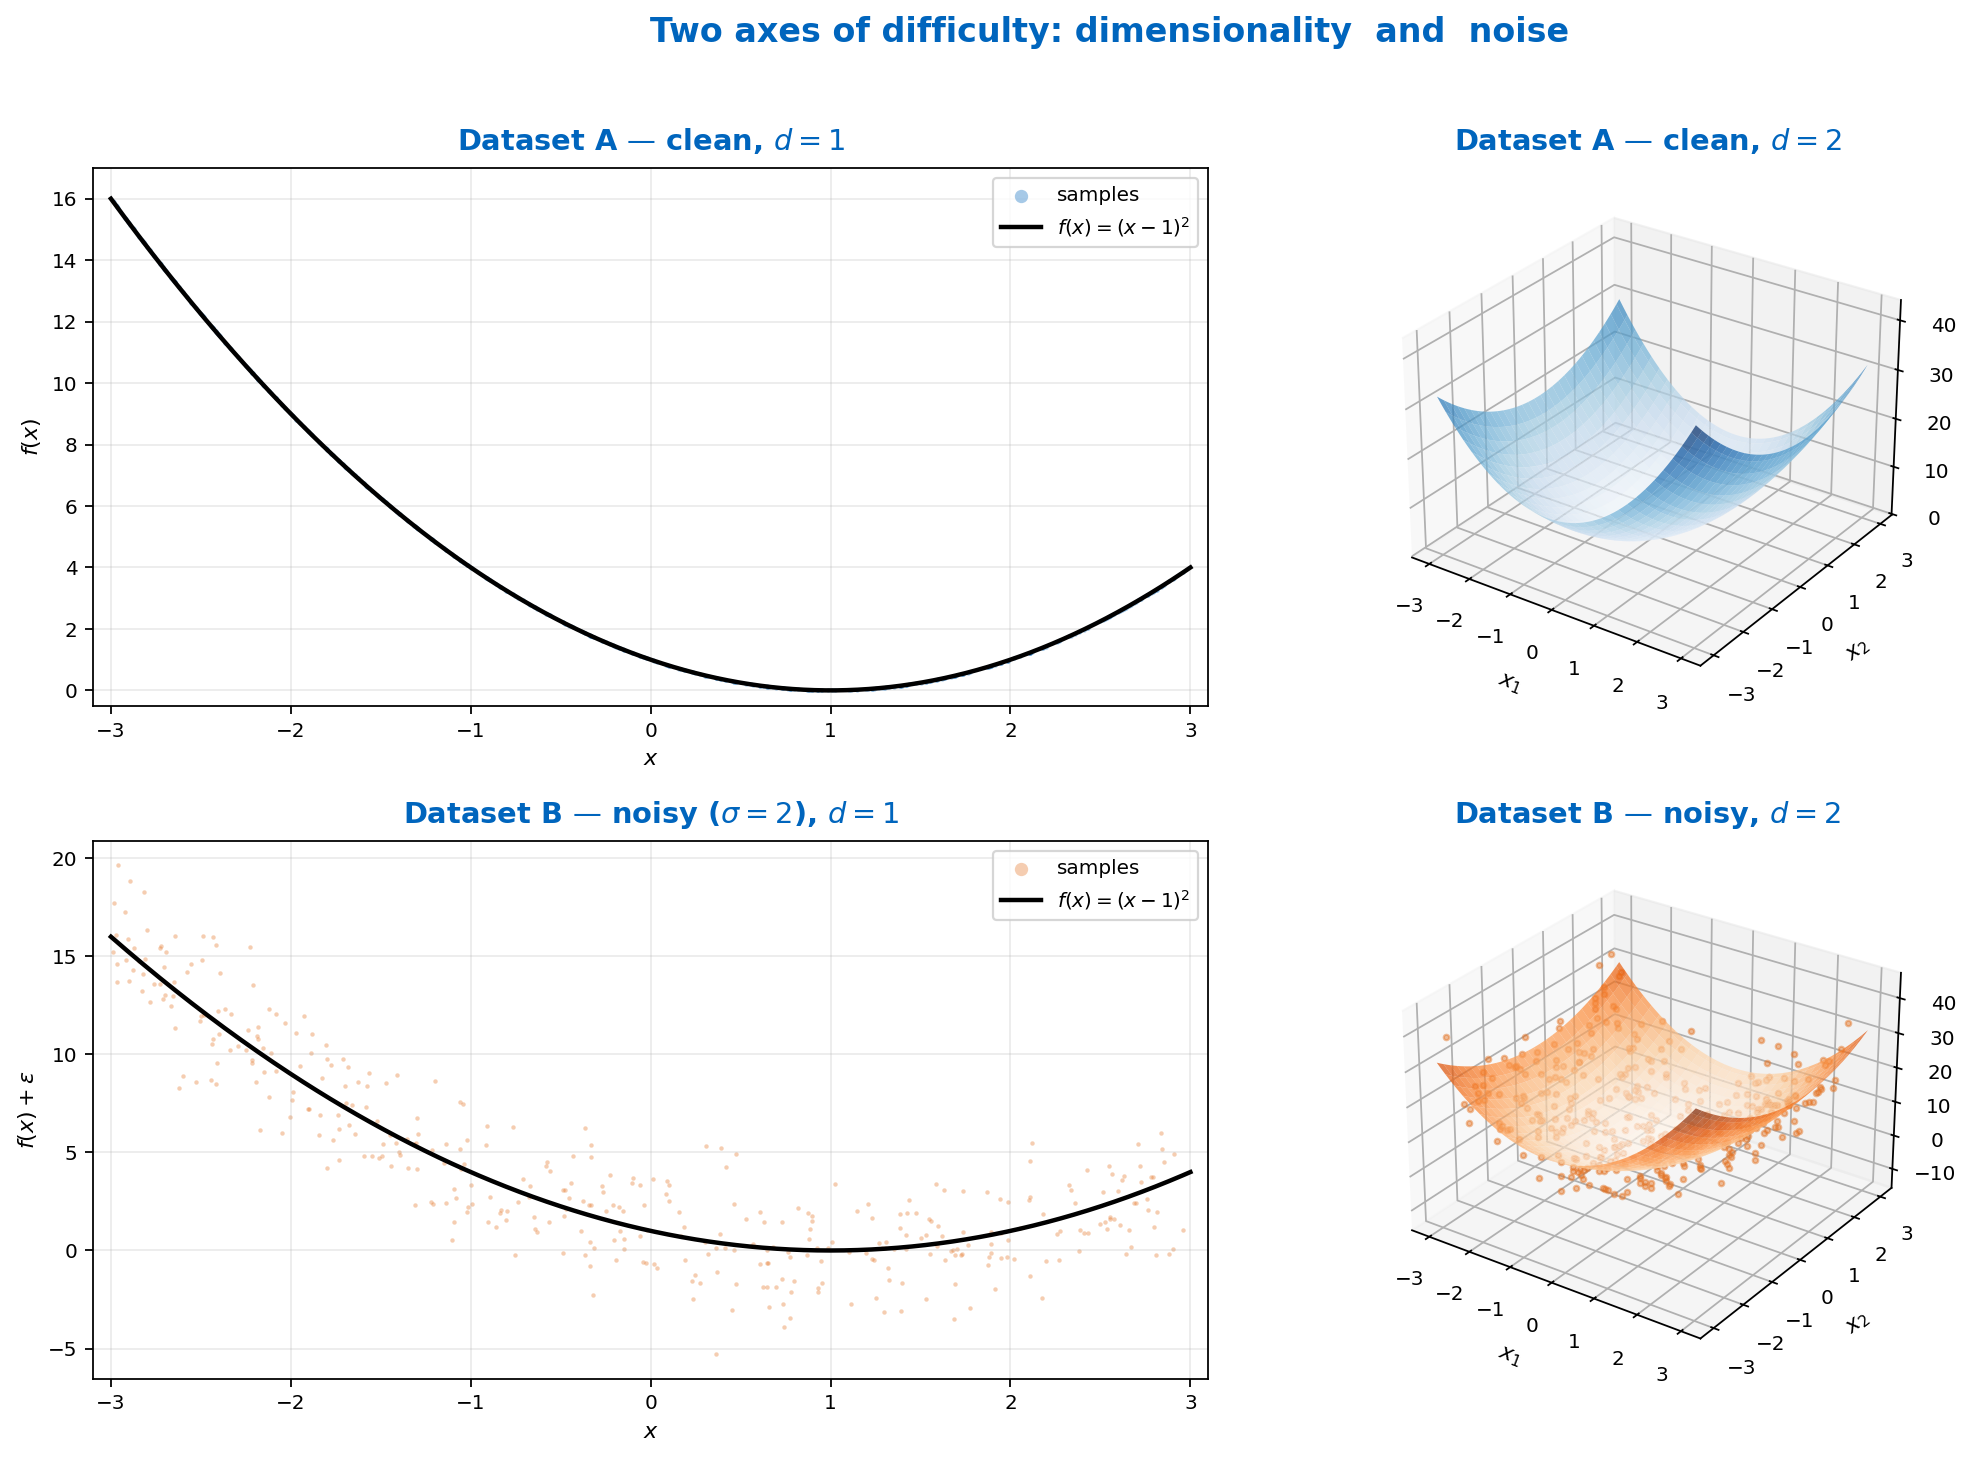
\includegraphics[width=0.96\linewidth]{dataset_viz_poster}
  \end{tikzfigure}
  \vspace{0.15em}
  {\small
  \textbf{A (clean):}
  $f(\mathbf{x}){=}(\mathbf{x}{-}\mathbf{1})^2$,
  $N{=}5\,000$, $\mathbf{x}\!\in\![-3,3]^d$.
  Extended to $d{=}2,3$ via a Cholesky-based SPD quadratic.
  Near-zero residual is achievable; the 3-D surface panel
  shows the exact ground truth for $d{=}2$.

  \vspace{0.2em}
  \textbf{B (noisy):} Same $f$ plus
  $\varepsilon\!\sim\!\mathcal{N}(0,\sigma^2)$,
  $\sigma{=}12.5\%$ of peak-to-peak range.
  The noise sets an irreducible MSE floor visible in the
  orange scatter panels.}
}

%% ---- METHODS -----------------------------------------------
\block{Methods: Pruning \& Topology Discovery}{

{\small
Nine methods \textbf{prune} a pre-trained (or newly initialised) network
by removing weights, neurons, or singular values.
The tenth, \textbf{ADAGOS}, is \emph{constructive}: it grows a compact
topology from scratch, never starting from a dense network.
Only OBD and OBS exploit second-order curvature information;
all others are first-order or gradient-free.
}

\vspace{0.4em}
{\small
\renewcommand{\arraystretch}{1.10}
\setlength{\tabcolsep}{2.5pt}
\begin{center}
\begin{tabular}{lllcp{6.5cm}r}
\toprule
\textbf{Method} & \textbf{Removes} &
\textbf{When?} & \textbf{2\textsuperscript{nd}~ord.} &
\textbf{Saliency / criterion} & \textbf{Ref.} \\
\midrule
\multicolumn{6}{l}{\textit{Post-training subtractive}} \\[1pt]
OBD        & weights & post & \checkmark
  & $\tfrac{1}{2}H_{ii}w_i^2$ & {[1]} \\
OBS        & weights & post & \checkmark
  & $\tfrac{w_q^2}{2[H^{-1}]_{qq}}$, rank-1 weight correction & {[2]} \\
Magnitude  & weights & post & $\times$
  & $|w_i|$ & --- \\
Taylor~FO  & weights & post & $\times$
  & $|w_i\nabla_{w_i}\mathcal{L}|$ & --- \\
Structured & neurons & post & $\times$
  & $\|\mathbf{w}_j^{\mathrm{out}}\|_2$ per neuron & --- \\
Activation & neurons & post & $\times$
  & $\mathrm{mean}|h_j(x)|$ per neuron & --- \\
Redundancy & neurons & post & $\times$
  & $|\rho_{ij}|>0.99$, merge correlated pairs & --- \\
Low-Rank   & sing.~vals & post & $\times$
  & Truncate smallest singular values of $W_\ell$ & --- \\
\midrule
\multicolumn{6}{l}{\textit{During / before training}} \\[1pt]
SNIP       & weights & at init & $\times$
  & Connection sensitivity $|w_i\nabla_{w_i}\mathcal{L}|_{t=0}$ & {[5]} \\
IMP+Rewind & weights & iterative & $\times$
  & $|w_i|$, rewind weights to early checkpoint & {[4]} \\
\midrule
\multicolumn{6}{l}{\textit{Constructive — topology search (patent)}} \\[1pt]
ADAGOS     & nodes/edges & joint & $\times$
  & Lagrangian error estimate; topology \emph{discovered} & {[6]} \\
\bottomrule
\end{tabular}
\end{center}
}
}

%% ============================  RIGHT  (48 %)
\column{0.48}

%% ---- EXPERIMENTAL SETUP ------------------------------------
\block{Experimental Setup}{

\textbf{Post-training methods.}
Baseline MLPs selected by Optuna TPE (up to 240 trials);
smallest model within 5\% of best validation MSE.
Fine-tuning after each pruning step follows
Augasta \& Kathirvalavakumar (2013)\,[3].

\vspace{0.4em}
{\small\setlength{\tabcolsep}{4pt}
\begin{center}
\begin{tabular}{llcrrc}
\toprule
\textbf{DS} & $d$ & \textbf{Architecture} &
\textbf{Params} & \textbf{FLOPs} & \textbf{Test MSE} \\
\midrule
A & 1 & $2{\times}16$, ReLU  &    321 &     609 & $1.94\times10^{-4}$ \\
A & 2 & $3{\times}32$, GELU  & 2\,241 &   4\,385 & $1.35\times10^{-3}$ \\
A & 3 & $3{\times}48$, GELU  & 4\,945 &   9\,745 & $4.19\times10^{-2}$ \\
\midrule
B & 1 & $1{\times}16$, ReLU  &     49 &      81 & $3.99$ \\
B & 2 & $2{\times}10$, ReLU  &    151 &     281 & $28.4$ \\
B & 3 & $2{\times}4$,  ReLU  &     41 &      73 & $625$ \\
\bottomrule
\end{tabular}
\end{center}
}

\vspace{0.45em}
\textbf{During/before-training methods.}
\textbf{SNIP}\,[5] masks weights at initialisation using connection
sensitivity ($|w_i\nabla_{w_i}\mathcal{L}|$ at $t{=}0$) — no
pre-training needed.
\textbf{IMP+Rewind}\,[4] iterates magnitude pruning with weight
rewinding to an early checkpoint (Lottery Ticket Hypothesis).

\vspace{0.45em}
\textbf{ADAGOS}\,[6] (US12124779B2): topology discovered jointly
with weights, starting from a minimal seed network:

\vspace{0.35em}
\begin{center}
\begin{tikzpicture}[node distance=0.85cm and 1.2cm]
  \node[adabox] (seed) {Seed\\[-2pt]network};
  \node[adabox, right=of seed] (add)  {Additive\\[-2pt]phase};
  \node[adabox, right=of add]  (sub)  {Subtractive\\[-2pt]phase};
  \node[adabox, right=of sub]  (stop) {Converged\\[-2pt]topology};
  \draw[adaarr] (seed) -- (add);
  \draw[adaarr] (add)  -- node[above,font=\scriptsize]{score} (sub);
  \draw[adaarr] (sub)  -- (stop);
  \draw[adaarr] (sub.south) -- ++(0,-0.75) -| (add.south)
    node[midway,below,font=\scriptsize]{iterate};
\end{tikzpicture}
\end{center}
}

%% ---- RESULTS -----------------------------------------------
\block{Results: Max Sparsity at $\leq\!1.5\times$ Baseline MSE}{

\noindent
\begin{minipage}[t]{0.49\linewidth}
\centering\textbf{Dataset A (clean)}\par\vspace{0.3em}
\begingroup
\renewcommand{\arraystretch}{2.3}%
\setlength{\tabcolsep}{4pt}%
\begin{tabular}{lrrr}
\toprule
\textbf{Method} & $d{=}1$ & $d{=}2$ & $d{=}3$ \\
\midrule
OBD        & \HiC{70}{1.30}{0.32F} & \LoC{30}{1.34}{0.70F} & \HiC{90}{0.63}{0.10F} \\
OBS        & \BestC{70}{1.01}{0.32F}& \NAC                  & \HiC{90}{0.63}{0.10F} \\
Magnitude  & \MiC{60}{1.26}{0.43F} & \HiC{70}{0.27}{0.30F} & \HiC{70}{0.37}{0.30F} \\
Taylor FO  & \MiC{50}{1.20}{0.48F} & \BestC{80}{0.80}{0.20F}& \BestC{90}{0.61}{0.10F} \\
SNIP       & \NAC                  & \NAC                  & \HiC{70}{1.47}{0.30F} \\
IMP+Rewind & \NAC                  & \HiC{70}{0.81}{0.30F} & \HiC{80}{1.26}{0.20F} \\
Structured & \MiC{50}{1.43}{0.48F} & \LoC{20}{1.15}{0.80F} & \MiC{40}{1.21}{0.60F} \\
Activation & \LoC{30}{1.14}{0.69F} & \MiC{60}{0.92}{0.40F} & \HiC{80}{0.98}{0.20F} \\
Redundancy & \LoC{20}{1.27}{0.79F} & \HiC{80}{0.50}{0.21F} & \HiC{70}{0.69}{0.30F} \\
Low-Rank   & \LoC{11}{1.01}{1.00F} & \LoC{10}{1.40}{1.00F} & \LoC{10}{1.02}{1.00F} \\
\bottomrule
\end{tabular}
\endgroup
\end{minipage}\hfill
\begin{minipage}[t]{0.49\linewidth}
\centering\textbf{Dataset B (noisy)}\par\vspace{0.3em}
\begingroup
\renewcommand{\arraystretch}{2.3}%
\setlength{\tabcolsep}{4pt}%
\begin{tabular}{lrrr}
\toprule
\textbf{Method} & $d{=}1$ & $d{=}2$ & $d{=}3$ \\
\midrule
OBD        & \HiC{90}{1.37}{0.31F} & \HiC{80}{1.01}{0.25F} & \BestC{70}{1.19}{0.37F} \\
OBS        & \HiC{80}{1.06}{0.41F} & \HiC{70}{1.00}{0.32F} & \MiC{50}{1.03}{0.59F} \\
Magnitude  & \BestC{90}{1.37}{0.28F}& \HiC{80}{1.09}{0.25F} & \MiC{60}{1.49}{0.48F} \\
Taylor FO  & \HiC{70}{1.01}{0.43F} & \BestC{90}{1.45}{0.15F}& \MiC{50}{1.01}{0.56F} \\
SNIP       & \HiC{90}{1.33}{0.31F} & \HiC{80}{1.43}{0.23F} & \MiC{60}{1.45}{0.42F} \\
IMP+Rewind & \HiC{80}{1.05}{0.38F} & \HiC{90}{1.45}{0.16F} & \LoC{30}{1.02}{0.75F} \\
Structured & \HiC{90}{1.24}{0.26F} & \HiC{90}{1.28}{0.15F} & \MiC{40}{1.00}{0.53F} \\
Activation & \HiC{90}{1.23}{0.26F} & \HiC{80}{1.43}{0.17F} & \HiC{70}{1.05}{0.32F} \\
Redundancy & \HiC{80}{1.37}{0.31F} & \HiC{70}{1.23}{0.34F} & \MiC{50}{1.18}{0.59F} \\
Low-Rank   & \LoC{0}{1.00}{1.00F}  & \LoC{8}{1.00}{1.00F}  & \LoC{12}{1.00}{1.00F} \\
\bottomrule
\end{tabular}
\endgroup
\end{minipage}

\vspace{0.3em}
{\small
\colorbox{CellHi}{\phantom{x}}~$\geq\!70\%$\enspace
\colorbox{CellMi}{\phantom{x}}~$40$--$60\%$\enspace
\colorbox{CellLo}{\phantom{x}}~$\leq\!30\%$/N/A\enspace
\colorbox{CellBest}{\color{white}\phantom{x}}~best\quad
\textit{Each cell:\ sparsity | MSE${\times}$baseline | FLOPs${\times}$baseline}}

\vspace{0.4em}
{\small\textbf{Key findings.}
\textbf{Taylor~FO} and \textbf{OBD} are the top scalers on
Dataset~A, both reaching 90\% at $d{=}3$ with MSE $\approx0.6\times$
baseline — larger networks prove proportionally more compressible.
On Dataset~B the noise floor dominates: most methods achieve 80–90\%
sparsity at $d{=}1,2$ with near-zero MSE penalty;
\textbf{Magnitude} leads at $d{=}1$ (0.28F), \textbf{Taylor~FO}
at $d{=}2$ (0.15F).
The \textbf{regularisation effect} on Dataset~A: Magnitude at 70\%
sparse on $d{=}2$ achieves $0.27\times$ baseline MSE.
\textbf{Low-Rank} fails in every setting; crucially,
FLOPs${\times}$\textbf{1.00} even at maximum truncation confirms it
provides zero inference speedup.
OBS degrades at $d{=}2$ (ill-conditioned $2241{\times}2241$ Hessian).}

\vspace{0.55em}
\begin{center}
\begin{tikzpicture}[scale=1.05]
  %% hidden-layer y positions: 4 neurons + midpoint vdots
  %% neurons at indices 1,2,4,5; vdots at index 3
  %% --- BEFORE ---
  \node[neuron, label={[font=\small]left:$x_1$}] (Bi1) at (0, 0.7) {};
  \node[neuron, label={[font=\small]left:$x_2$}] (Bi2) at (0,-0.7) {};
  \foreach \i/\y in {1/2.1, 2/0.7, 4/-0.7, 5/-2.1}
    \node[neuron] (Ba\i) at (2.4,\y) {};
  \node[font=\normalsize] at (2.4,0) {$\vdots$};
  \foreach \i/\y in {1/2.1, 2/0.7, 4/-0.7, 5/-2.1}
    \node[neuron] (Bb\i) at (4.8,\y) {};
  \node[font=\normalsize] at (4.8,0) {$\vdots$};
  \foreach \i/\y in {1/2.1, 2/0.7, 4/-0.7, 5/-2.1}
    \node[neuron] (Bc\i) at (7.2,\y) {};
  \node[font=\normalsize] at (7.2,0) {$\vdots$};
  \node[neuron, label={[font=\small]right:$\hat{y}$}] (Bo) at (9.6,0) {};
  %% all connections (before = dense)
  \foreach \inp in {Bi1,Bi2} \foreach \i in {1,2,4,5}
    { \draw[active] (\inp)--(Ba\i); }
  \foreach \i in {1,2,4,5} \foreach \j in {1,2,4,5}
    { \draw[active] (Ba\i)--(Bb\j); }
  \foreach \i in {1,2,4,5} \foreach \j in {1,2,4,5}
    { \draw[active] (Bb\i)--(Bc\j); }
  \foreach \i in {1,2,4,5} { \draw[active] (Bc\i)--(Bo); }
  \node[font=\small\bfseries\color{TUMblue}] at (4.8,3.1)
    {Before ($d{=}2$, $3{\times}32$)};

  %% --- ARROW ---
  \draw[-{Stealth[length=10pt]}, line width=2.8pt, TUMorange]
    (10.4,0) -- node[above,font=\normalsize\bfseries\color{TUMorange}]
    {\,prune\,} (11.8,0);

  %% --- AFTER ---
  \node[neuron, label={[font=\small]left:$x_1$}] (Ai1) at (12.6, 0.7) {};
  \node[neuron, label={[font=\small]left:$x_2$}] (Ai2) at (12.6,-0.7) {};
  \foreach \i/\y in {1/2.1, 2/0.7, 4/-0.7, 5/-2.1}
    \node[neuron] (Aa\i) at (15.0,\y) {};
  \node[font=\normalsize] at (15.0,0) {$\vdots$};
  \foreach \i/\y in {1/2.1, 2/0.7, 4/-0.7, 5/-2.1}
    \node[neuron] (Ab\i) at (17.4,\y) {};
  \node[font=\normalsize] at (17.4,0) {$\vdots$};
  \foreach \i/\y in {1/2.1, 2/0.7, 4/-0.7, 5/-2.1}
    \node[neuron] (Ac\i) at (19.8,\y) {};
  \node[font=\normalsize] at (19.8,0) {$\vdots$};
  \node[neuron, label={[font=\small]right:$\hat{y}$}] (Ao) at (22.2,0) {};
  %% all connections pruned first
  \foreach \inp in {Ai1,Ai2} \foreach \i in {1,2,4,5}
    { \draw[pruned] (\inp)--(Aa\i); }
  \foreach \i in {1,2,4,5} \foreach \j in {1,2,4,5}
    { \draw[pruned] (Aa\i)--(Ab\j); }
  \foreach \i in {1,2,4,5} \foreach \j in {1,2,4,5}
    { \draw[pruned] (Ab\i)--(Ac\j); }
  \foreach \i in {1,2,4,5} { \draw[pruned] (Ac\i)--(Ao); }
  %% ~13 surviving out of 44 ≈ 70% pruned
  \draw[active] (Ai1)--(Aa1);   \draw[active] (Ai1)--(Aa2);
  \draw[active] (Ai2)--(Aa4);   \draw[active] (Ai2)--(Aa5);
  \draw[active] (Aa1)--(Ab2);   \draw[active] (Aa2)--(Ab1);
  \draw[active] (Aa4)--(Ab4);   \draw[active] (Aa5)--(Ab5);
  \draw[active] (Ab1)--(Ac1);   \draw[active] (Ab2)--(Ac2);
  \draw[active] (Ab4)--(Ac5);   \draw[active] (Ab5)--(Ac4);
  \draw[active] (Ac1)--(Ao);    \draw[active] (Ac4)--(Ao);
  \node[font=\small\bfseries\color{TUMblue}] at (17.4,3.1)
    {After (${\approx}70\%$ sparse)};
  %% legend
  \draw[active]  (13.0,-3.2) -- +(1.2,0)
    node[right,font=\small]{surviving};
  \draw[pruned]  (17.0,-3.2) -- +(1.2,0)
    node[right,font=\small]{pruned};
\end{tikzpicture}
\end{center}
}

\end{columns}

\begin{columns}
  \column{1.0}
  \block{References}{
  {\small
  \begin{minipage}[t]{0.46\linewidth}
  \begin{enumerate}[leftmargin=1.6em, itemsep=0.1em]
    \item LeCun, Denker \& Solla (1990).
          \textit{Optimal Brain Damage.} NeurIPS.
    \item Hassibi \& Stork (1993).
          \textit{Second-Order Derivatives for Network Pruning:
          Optimal Brain Surgeon.} NeurIPS.
    \item Augasta \& Kathirvalavakumar (2013).
          \textit{Pruning algorithms of neural networks --- a
          comparative study.} CSIT.
  \end{enumerate}
  \end{minipage}\hfill
  \begin{minipage}[t]{0.46\linewidth}
  \begin{enumerate}[leftmargin=1.6em, itemsep=0.1em, start=4]
    \item Frankle \& Carlin (2019).
          \textit{The Lottery Ticket Hypothesis.} ICLR.
    \item Lee et al.\ (2019).
          \textit{SNIP: Single-shot Network Pruning based on
          Connection Sensitivity.} ICLR.
    \item Bompard et al.\ (2024).
          \textit{Method of neural network construction for the
          simulation of physical systems.} US12124779B2.
  \end{enumerate}
  \end{minipage}
  }}
\end{columns}

\end{document}
